\section{Evaluation}

\comment{

Giza provides fault tolerance through erasure coding across wide area networks while providing linearizability for its read and write operations. As such, there are currently no system that is specifically designed to serve as an alternative to Giza. However, we benchmark Giza’s performance against Cassandra and CockroachDB to illustrate the following points:

- In the common case, Giza’s Fast Paxos implementation of the metadata phase allows for lower latency writes for Giza when compared to Cassandra.

- While one could implement Giza’s metadata phase and data phase as a single distributed transaction, we illustrate through CockroachDB that doing so will degrade performance significantly.

In addition, we provide evaluation results for encoding scheme ranging from 2-1 in 3 data centers to 18-4 in 22 data centers to illustrate the flexibility of Giza as a front end.

}

For evaluation, we deploy Giza on top of the Microsoft Azure platform. The deployment reaches xxx data centers (xxx in North America, xxx in Europe and xxx in Asia). In each data center, we create a set of virtual machines as Giza nodes. We also create a number of Azure storage accounts. These storage accounts are local to individual DCs and allow access to Azure Blob storage and Azure Table storage in the DCs.

We form \name storage account as a collection of the local Azure storage accounts. We also specify the erasure coding scheme for each account. For example, a North American only Giza storage account may apply $2+1$ erasure coding and consist of 4 data centers in the US, as xxx, xxx, xxx and xxx. A global Giza storage account may apply same coding and consist of 4 data centers across 3 continents, as xxx, xxx, xxx and xxx.

As described in section~\ref{sec:design}, all the Giza nodes are stateless. Upon receiving {\em get} or {\em put} requests, the Giza nodes execute the data and the metadata paths to read or write data objects.

\begin{figure*}
\begin{tabular}{c|c|c|c|c|c}
& coding rate & \# of DCs & DC location & Max Metadata Latency & Max Latency\\
\hline
US-2-1 & 2+1 & 4 & Central, South Central, West & 40 ms& 40 ms\\
US-6-1 & 6+1 & 8 & Central, South Central, West&?? 40 ms&?? 42 ms\\ 
world-2-1 & 2+1 & 4 & Central, Europe North, Japan East & 140 ms & 140 ms\\
world-6-1 & 6+1 & 8 & Central, South Central, West & 40 ms & 140 ms\\
\end{tabular}
\caption{The DC configurations and inter-DC latencies in various experiments~\label{fig:dcconfig}} 
\end{figure*}

\subsection{Setup}
Our experiments involve a varying number of DCs in different configurations. In
each DC, we deploy a single Azure virtual machine (16 cores, 56 GB of RAM, and
gigabit ethernet) and create a storage account for accessing Azure blob and
table storage. Both the blob and table storage are configured with the
``locally redundant'' replication level.  Each \name node accesses the local
DC's cloud storage and also proxies the storage requests from \name nodes in
other DCs.  

For CockroachDB experiments, we run a CockroachDB cluster spanning across
multiple DCs.  We use the same set of Azure virtual machines and run a single
CockroachDB node per DC. Our configuration of CockroachDB follows the
recommended production settings by the developers of CockroachDB. For example,
we run NTP to synchronize the clocks of different CockroachDB nodes. 

We generate experimental workloads using the YCSB benchmark. In the generated
workload, the probability of accessing a given key follows a Zipf distribution.
We experiment with different object sizes ranging from 128KB to 4MB. 

We experiment with four diffferent DC configurations, as shown in
Figure~\ref{fig:dcconfig}.  These configurations correspond to different coding
rates and different choices of DCs, either within US-only or spread across the
world. The wide-area latency across different DCs plays an important role in 
the performance of \name.  Figure~\ref{fig:dcconfig} reports the majority
latency (measured as the latency required to get a response from a majority
quorum of DCs) and the maximum latency between DCs.


\subsection{Metadata Path Optimization}
\sm {
  Hey Shuai, here I will provide the graph compaing the two metadata paths and the datapath to illustrate that this optimization makes the metadata path the non-dominant path in most cases. I will also have a table with the latency breakdown. The motivation for this is to show that such an optimization can allow users to tune the latency performance by changing the erasure coding scheme. This would not be possible it we use the two round trip. I will provide different latency measurements (95th, 75th, 50th percentile, as well as average with error bar so we can choose one later. This is true for all latency results I will provide)
}
We measure Giza's latency performance by running 1000 write and read operations with a single threaded Giza node.We vary the object size (1mb and 4mb) and compared different configurations. 
The 95th percentile latency result is shown in Figure 4. The four configurations we chose are 3 data centers in the US (2-1 erasure coding scheme), 3 data centers across the world, 7 data centers in the US (6-1 erasure coding scheme), and 7 data centers across the world. Both the configuration (i.e distance between data centers) and the size of the object impact latency peformance. Larger objects incur higher latency in both the vm to vm transfer and the local blob storage access. This can explain the similar put latency results between the 3 US data center configuration and the 7 US data center configuration. Even though in the 3 US data center configuration, the distance between the data centers are much shorter (Iowa, Illinois, and West Central), each data fragment is 2MB. We can see in Table 3 that this increases the latency performance for the data path. In the 7 US data center configuration, each data fragment is just 700 KB, which reduces latency even when the data centers are further away. 

}

\subsection{Decomposing \name Latencies}

In our workloads, the predominant object size is 4MB. Hence, we focus on the {\em put} and {\em get} latency of 4MB objects in the evaluation. For every data point reported in this section, we repeat the corresponding Giza operation 1000 times and then calculate the latency at desired percentile. The global Giza storage account with 4 DCs is used for this evaluation.

\subsubsection{Data Path Tunneling}

\Cref{fig:eval_tunneling} shows the latency comparison between data path with tunneling and 
directly accessing remote blob storage without tunneling. The median latency with tunneling 
is xxx ms, vs xxx ms without tunneling. In addition, the latency with tunneling is much 
more stable over time. Its (90\%, 10\%) latency is (xxx ms, xxx ms), while without tunneling 
is (xxx ms, xxx ms). The variance without tunneling probably comes from the blob storage 
has a huge public load and it varies over time. Although in practice \name without tunneling 
should bring the same level of performance improvement, we chose tunneling for the rest of 
the evaluation to have more analysis-friendly results.

\subsubsection{Metadata Path}

To show the effects of our fast path design of metadata, we mesured the metadata path latency 
for both fast path and slow path, as shown in~\Cref{fig:eval_fastpath}. As expected, the fast 
path takes one network roundtrip plus the table read/write latency (with median at xxx ms); 
the slow path takes two roundtrips, whose latency is about twice of fast path (with median at 
xxx ms). This test concludes that the fast path optimization is critical to \name overall 


%\subsubsection{Giza Put Latency}
\subsubsection{Giza Latency}

\Cref{fig:eval_giza_put} shows the \name overall put latency for 4MB data. In comparison, 
we tested two possible alternative designs: a sequential datapath with slow metadata 
path (as normal Paxos); parallel datapath with slow metadata path. In addition, we also 
included a one across datacenter RPC plus blob storage access test as baseline (it does 
not gurantee any level of consistency).

The results show that \name's performance beats the other two alternatives and has closest
latency to the baseline. The median latency of \name put is xxx ms, which is only xxx ms
higher than the baseline. On the other hand, the serial version with only slow path takes 
xxx ms, and the parallel version with slow path takes xxx ms.

Similar to the put test, we did a \name get test, as shown in~\Cref{fig:eval_giza_get}. 
\name also beats the other two alternatives, with a median latency xxx ms, higher than 
the baseline by xxx ms. The gap between \name and baseline is higher because in the get 
operation \name needs to do a local table retrieve first before starting the datapath. 

%The results are expected. The \name put latency consists of a 
%metadata put latency and datapath latency. 

%\subsubsection{Giza Read Latency}



\comment{

% \begin{figure}[!h]
% \centering
%   \subfloat[Giza Put 99th Percentile]{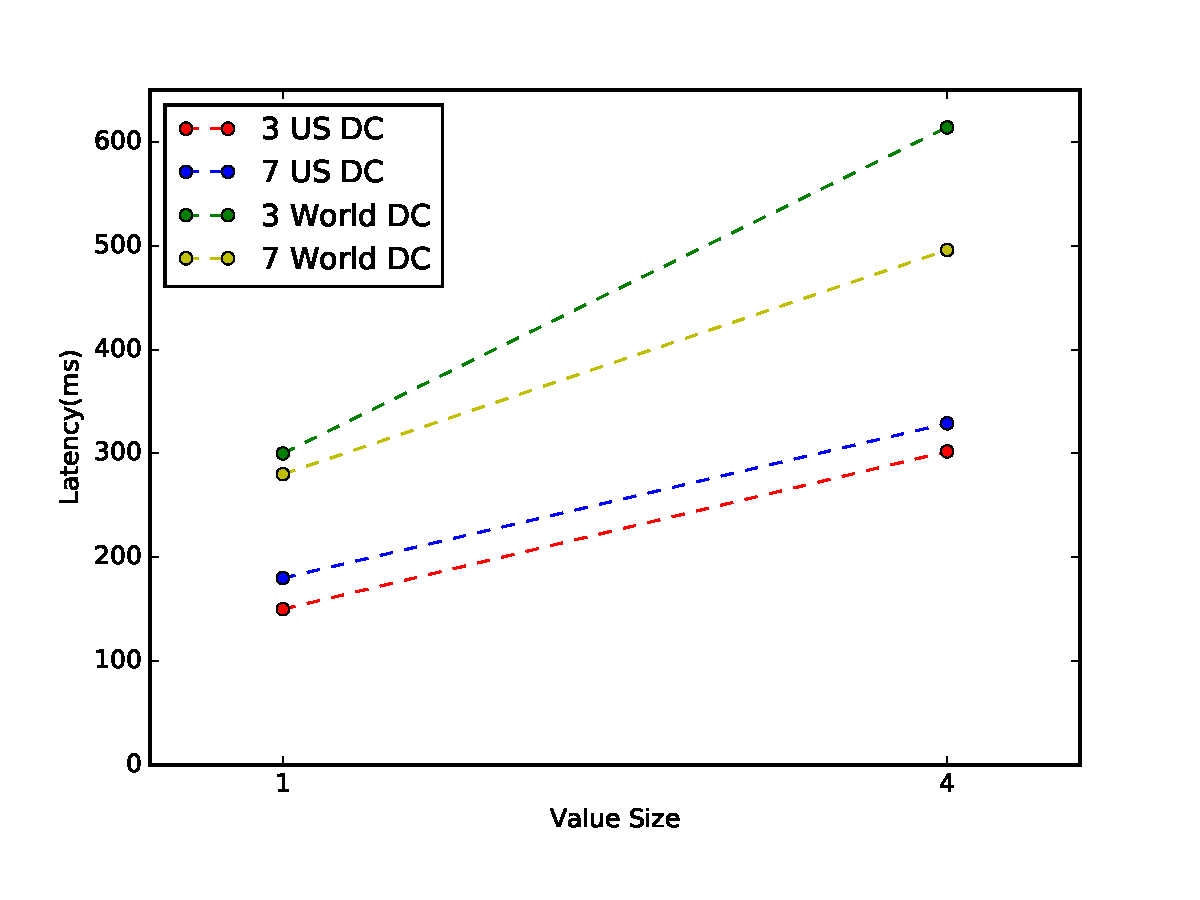
\includegraphics[width=0.5\textwidth]{images/write_latency}\label{fig:f1}}
%   \subfloat[Giza Get 99th Percentile]{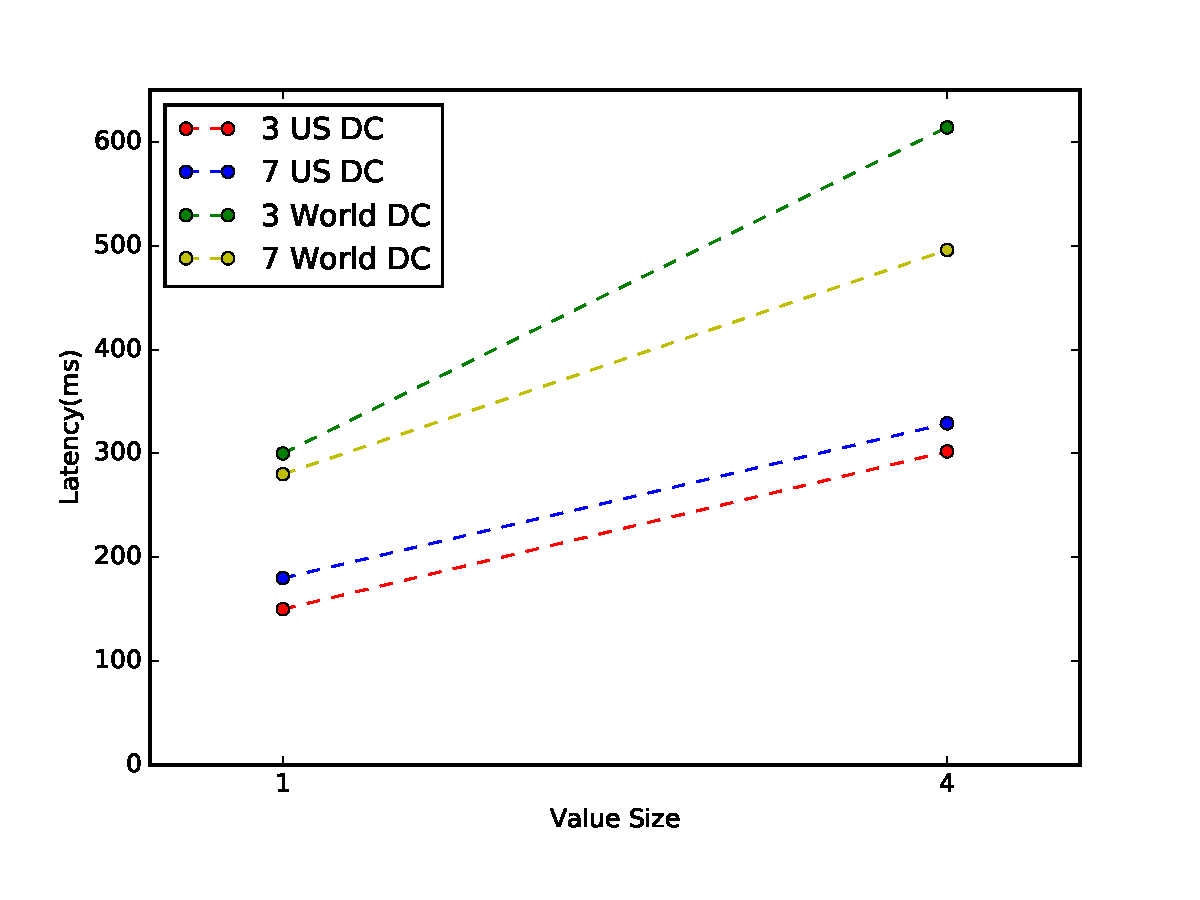
\includegraphics[width=0.5\textwidth]{images/write_latency}\label{fig:f2}}
% \caption{Comparison of latency of the four configurations}
% \end{figure}
\subsection {Different Configurations}
\sm {
  In this section, I will provide a latency graph (put and get) of all the 4 different configurations. The x axis is the size of the objects and the y axis is the latency. This section is to illustrate the trade off between storage efficiency and read latency. 
}

}

\subsection{Footprint Impact}


\begin{figure}[t]
%  \centerline {
    \begin{subfigure}{0.40\textwidth}
      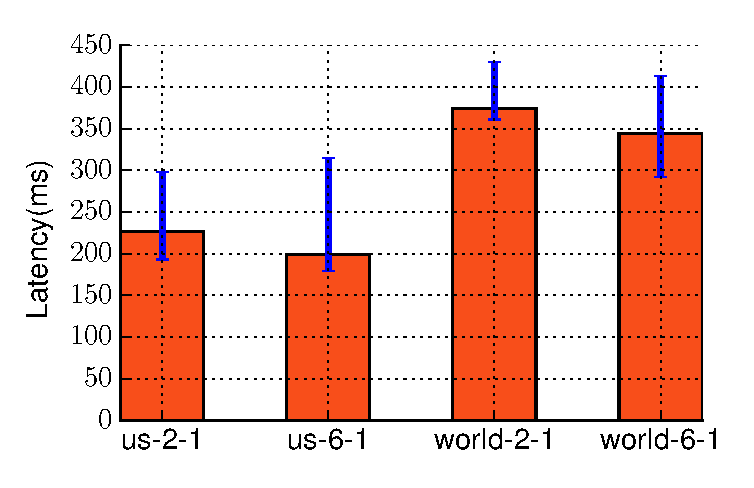
\includegraphics[width=\linewidth]{plots/giza_four_put}

      % \placeholder{
      %   x-axis: \# clients / partition\\
      %   y-axis: cluster throughput\\
      %   lines: \name{}, OCC, 2PL, TAPIR\\
      %   }
%                \vspace{-1\baselineskip}
      \caption{Put}
      \label{fig:eval_giza_put_four}
    \end{subfigure}
%    \begin{subfigure}{0.33\textwidth}
%      \includegraphics[width=\linewidth]{figs/graphs/multi_dc/tpcc/tpcc_NEW_ORDER_tpcc_client_lat90.eps}
%
%      % \placeholder{
%      %   x-axis: \# clients / partition\\
%      %   y-axis: latency (median, p90, p99)\\
%      %   (maybe only show median and p99 or just median and report typical distribution)\\
%      %   lines: \name{}, OCC, 2PL, TAPIR\\
%      % }
%      \caption{90\% Latency}
%      \label{fig:geo_tpcc_latency}
%    \end{subfigure}
    \begin{subfigure}{0.40\textwidth}
      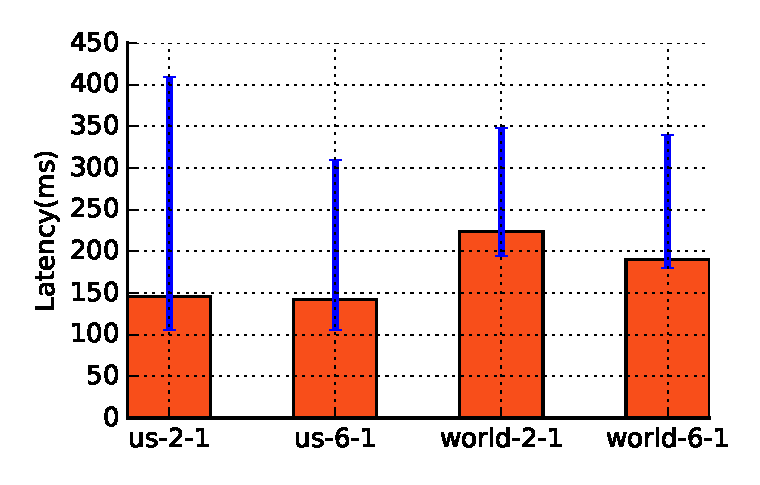
\includegraphics[width=\linewidth]{plots/giza_four_get}

      % \placeholder{
      %   x-axis: \# clients / partition\\
      %   y-axis: commit rate\\
      %   lines: \name{}, OCC, 2PL, TAPIR\\
      % }
      %\includegraphics[width=\linewidth]{fig/kodiak/tpcc_mix_10_nlog_ct_cr.pdf}
%                \vspace{-1\baselineskip}
      \caption{Get}
      \label{fig:eval_giza_get_four}
    \end{subfigure}
%  }
  \caption{Performance for \name in different setups}
\end{figure}

%%% Local Variables:
%%% mode: latex
%%% TeX-master: "main"
%%% End:


\name offers customers the flexibility to choose the set of data centers, as well as the 
erasure coding schemes. To show the performance of different configurations, we evaluate 
4 different \name storage accounts, with the cross combination of $2+1$ vs $6+1$ erasure 
coding and all data centers in North America vs across 3 continents.

~\Cref{fig:eval_giza_put_four} shows the put latency for different configurations; 
~\Cref{fig:eval_giza_get_four} shows the get latency. When the system is deployed within 
North America, it has more stable latency results with both coding schemes. The $6+1$ coding
is faster because it gives more parallelism for the data path. Because the data is fixed, 
having more datacenters means smaller data fragments. The world-wide deploy shows much 
more invariance in performance, which is expected because the system is facing the across-
continent internet traffic. The $6+1$ performs better in this setup, in terms of the 
both median latency and variance. 


\subsection{Comparing Giza with CockroachDB}

%To set up CockroachDB, we use the same azure virtual machine instances and run a single CockroachDB node. We followed the recommended production settings by the developers of CockroachDB when deploying these instances. For example, on the same virtual machine, we also run NTP to provide moderately accurate time to preserve data consistency. Other optimizations can be found on the CockroachDB website. We only benchmark CockraochDB against Giza in the 3 dc cluster scenario since we want the fault tolerance level to be the same for the comparisons.
%Since variability in latency is a factor when benchmarking cloud storage, we run all our experiments at approximately the same time.
%Since latency is an issue, we run all our experiments at around the same time.
%We experimented with different erasure coding schemes
% For all experiments, we deployed a single virtual machine (16 cores, 56 GB of RAM, 800 GB SSD, and gigabit ethernet) for each geographical region. We use the same virtual machines for setting up the Cassandra and CockroachDB clusters. The client issuing the requests runs on one of the virtual machine that is also part of the cluster. 
% To set up Giza, we also had to deployed both a table service and a blob service provided by the cloud service platform. The granularity of replication for these services varies from provider to provider but we always choose the replication level to match that of the regional replication. This means that as long as there’s no dc outage, the data would not be lost. For each data center, we run a Giza node frontend with the virtual machine. The Giza node can service requests from a client running in the virtual machine. In addition, requests to its local table and blob storage from other Giza nodes also go through the Giza node frontend in the form of an RPC call. This is to avoid unecessary WAN round trips when dealing with complicated table and blob storage operations. 

\sm {
  In this section, I will have two graphs. One comparing Giza's full write path with CockroachDB's full replication. Another one is comparing the metadata path with cockroach db. This is to show, hopefully, that the fast paxos scheme is better. I will probably have 3 graphs each making request from one of the three datacenters. Due to multipaxos, there might be extra latency for cockroachdb's case.
}
We benchmark the performance of Giza with CockroachDB in two cases. In the first case, we use CockroachDB as a geo-replicating blah blah blah. Here is the result.
In the second case, we used cockroachdb's transaction to simulate what we are doing with Giza. Blah blah blah, here is the result.
64K $\sim$ 16MB

X-axis: Value size
Y-axis: 50\% Read latency

X-axis: Value size
Y-axis: 90\% Read latency

X-axis: Value size
Y-axis: 99\% Read latency

Same for write

[adding cpu results in a table]

% \subsection{Large object}
% 256MB $\sim$ 1GB

% X-axis: Value size
% Y-axis: Average Read latency

% X-axis: Value size
% Y-axis: Average Write latency


% \subsection{Contention}

% Fixed object size
% X-axis: zipf coefficient
% Y-axis: 50\%, 90\%, 99\% Read/Write Latency


% \subsection{Real workload}
% Table.


%%% Local Variables:
%%% mode: latex
%%% TeX-master: "main"
%%% End:

